\chapter{Plugin Implementation}
\label{sec:PluginImplementation}
In this chapter we provide step-by-step instructions for implementing your own CrypTool 2 plugin. We shall assume that you have already retrieved the CrypTool 2 source code from the SVN repository, set up Visual Studio 2010 or Visual C\# 2010 Express to build CrypTool 2, and you have placed the plugin template in the right place.

\section{Create a new project}
\label{sec:CreatingANewProject}

Open the CrypTool 2 solution, right click in the solution explorer on \textit{CrypPlugins} (or on the top solution item, if you're using Visual C\# Express) and select \textit{Add~$\rightarrow$ New Project}. In the dialog window, select \textit{Visual C\# $\rightarrow$ CrypTool 2.0 Plugin} as project template and enter a unique name for your new plugin project (such as \textit{Caesar} in our case). The \textbf{next step is crucial} to ensure that your plugin will compile and run correctly: select the subdirectory \texttt{CrypPluginsExperimental\textbackslash} as the location of your project (Figure~\ref{fig:vs_create_new_project}).

\begin{figure}[h!]
	\centering
		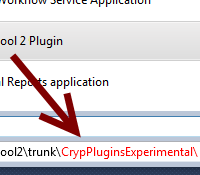
\includegraphics{figures/vs_create_new_project.png}
	\caption{Creating a new CrypTool 2 plugin project.}
	\label{fig:vs_create_new_project}
\end{figure}

As the project basics are already correctly set up in the template, you should now be able to compile the new plugin. First of all, rename the two files in the solution explorer to something more meaningful, for example \texttt{Caesar.cs} and \texttt{CaesarSettings.cs}.

\begin{figure}[h!]
	\centering
		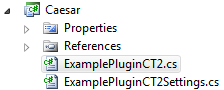
\includegraphics{figures/caesar_project.png}
	\caption{Items of a new plugin project.}
	\label{fig:caesar_project}
\end{figure}

\section{Adapt the plugin skeleton}
\label{AdaptingThePluginSkeleton}

If you look into the two C\# source files (Figure~\ref{fig:caesar_project}), you will notice a lot of comments marked with the keyword \texttt{HOWTO}. These are hints as to what you should change in order to adapt the plugin skeleton to your custom implementation. Most \texttt{HOWTO} hints are self-explanatory and thus we won't discuss them all.

\section{Defining the attributes of the Caesar class}
\label{sec:DefiningTheAttributesOfTheCaesarClass}

The next thing we will do in our example \textit{Caesar.cs} is define the attributes of our class. These attributes are used to provide necessary information for the CrypTool 2 environment. If they are not properly defined, your plugin won't show up in the application user interface, even if everything else is implemented correctly.

Attributes are used for declarative programming and provide metadata that can be added to the existing .NET metadata. CrypTool 2 provides a set of custom attributes that are used to mark the different parts of your plugin. These attributes should be defined right before the class declaration.

\subsection{The \protect\textit{[Author]} attribute}
\label{sec:TheAuthorAttribute}

The \textit{[Author]} attribute is optional, meaning that we are not required to define it. The attribute can be used to provide additional information about the plugin developer (or developers, as the case may be). This information will appear in the TaskPane. We will define the attribute to demonstrate how it should look in case you want to use it in your plugin.

\begin{figure}[h!]
	\centering
		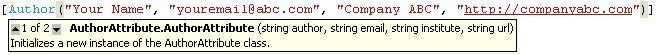
\includegraphics[width=.90\textwidth]{figures/attribute_author.jpg}
	\caption{The defintion for the \textit{[Author]} attribute.}
	\label{fig:attribute_author}
\end{figure}

All of these elements are optional and may be null:

\begin{itemize}
	\item \textit{Author} --- the name of the plugin developer.
	\item \textit{Email} --- the email address of the plugin developer, should he or she wish to be available for contact.
	\item \textit{Institute} --- the organization, company or university with which the developer is affiliated.
	\item \textit{URL} --- the website of the developer or of his or her institution.
\end{itemize}

\subsection{The \protect\textit{[PluginInfo]} attribute}
\label{sec:ThePluginInfoAttribute}

The \textit{[PluginInfo]} attribute provides necessary information about the plugin, and is therefore mandatory. The information defined in this attribute appears in the caption and tool tip window. The attribute is defined as follows:

\begin{figure}[h]
	\centering
		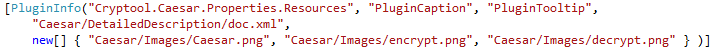
\includegraphics[width=1.00\textwidth]{figures/attribute_plugininfo.png}
	\caption{Multilingual defintion of \textit{[PluginInfo]} attribute.}
	\label{fig:attribute_plugininfo}
\end{figure}

\noindent This attribute has the following parameters:

\begin{itemize}
	\item \textit{Resource File} --- the namespace and class name of an associated resource file \textit{.resx}. This element is optional and used only if the plugin provides multilingual strings (see also Section~\ref{sec:Internationalization}).
	\item \textit{Caption} --- the name of the plugin, or, if using a resource file, the name of the field in the file with the caption data. This element is mandatory.
	\item \textit{ToolTip} --- a description of the plugin, or, if using a resource file, the name of the field in the resource file with the toolTip data. This element may be null.
	\item \textit{DescriptionURL} --- the local path of the user documentation file (XML file, see Section~\ref{sec:Documentation}). This element may be null.
	\item \textit{Icons} --- an array of strings to define all the paths of the icons used in the plugin (i.e.\ the plugin icon described in Section \ref{sec:AddingAnIconToTheCaesarClass}). This element may be null.
\end{itemize}

For your first plugin, it's recommended to skip the resource file and use English strings for \textit{Caption} and \textit{ToolTip}. If you're ready to add multi-language support to your plugin, take a look at Section~\ref{sec:Internationalization}.

The \textit{DescriptionURL} element defines the location path of the user documentation file (custom XML format), e.g. \texttt{"assemblyname/path/filename.xml"}. Take a look at Section~\ref{sec:Documentation} to see how to create a documentation file.

The \textit{Icons} parameter is an array of strings and should be provided in format: \\
\texttt{new[] \{ "assemblyname/path/filename.png" \} }

Don't forget to add all files to your project in Visual Studio. See Section~\ref{sec:AddingAnIconToTheCaesarClass} how to do this.

\subsection{Set algorithm category}
\label{sec:AlgorithmCategory}

In the CrypTool 2 user interface plugins are grouped by their algorithm category, for example hash function, symmetric cipher, and so on. To set the category, you must specifiy the attribute \textit{[ComponentCategory]}. Multiple categories are allowed.

\begin{lstlisting}
    [ComponentCategory(ComponentCategory.CiphersClassic)]
    public class ExamplePluginCT2 : ICrypComponent
		{
\end{lstlisting}

\subsection{Adding parameters to the CaesarSettings class}
\label{sec:AddingControlsToTheCaesarSettingsClass}

If your component provides user-configurable parameters, you can set them up in the settings class derived from \textit{ISetting}. This comprises text input fields, number fields, combo boxes, radio buttons and so on. Take a look at \textit{CaesarSettings.cs} to see some examples for user-configurable parameters.

If you don't want to provide any parameters, delete the class and return null for the \textit{Settings} property:

\begin{lstlisting}
	public ISettings Settings
	{
		get { return null; }
	}
\end{lstlisting}

\section{Add an icon file}
\label{sec:AddingAnIconToTheCaesarClass}

Your component is represented in the CrypTool 2 user interface by an icon. You should add a custom icon file, but if you don't, the template uses a generic default one.

The proper image size is 40x40 pixels, but since the image will be rescaled if necessary, any size is technically acceptable. Once you have saved your icon, you should add it directly to the project or to a subdirectory with it. Right-click on your plugin project or any subfolder and select \textit{Add $\rightarrow$ Existing Item}.

\begin{figure}[h!]
	\centering
		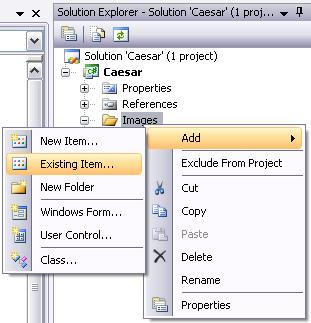
\includegraphics{figures/add_existing_item.jpg}
	\caption{Adding an existing item.}
	\label{fig:add_existing_item}
\end{figure}
\clearpage

Choose \textit{Image Files} as the file type and select your newly-created icon for your plugin.

\begin{figure}[h!]
	\centering
		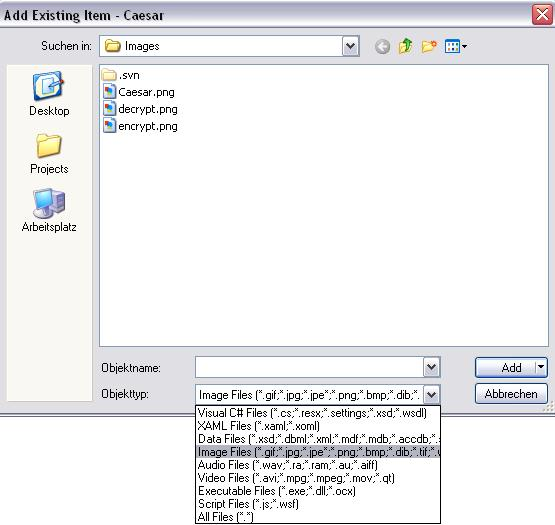
\includegraphics{figures/choose_icon.jpg}
	\caption{Selecting the image file.}
	\label{fig:choose_icon}
\end{figure}
\clearpage

It's \textbf{necessary} to set the icon file as a \textit{Resource} in the file properties. Right-click on your icon file, click \textit{Properties} and set the \textit{Build Action} to \textit{Resource}.

\begin{figure}[h!]
	\centering
		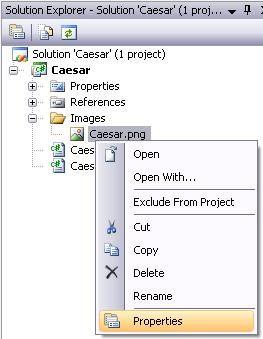
\includegraphics{figures/icon_properties.jpg} 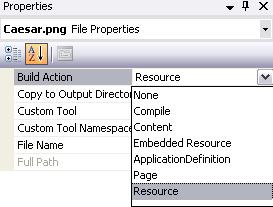
\includegraphics{figures/icon_build_action.jpg}
	\caption{Go to \textit{Properties}, select \textit{Build Action} to \textit{Resource}.}
	\label{fig:icon_properties}
\end{figure}

\section{Input and output dockpoints}
\label{sec:InputAndOutputDockpoints}

Next we will define some class properties to be used as data input and output connectors of the component. Each property is defined by a \textit{[PropertyInfo]} attribute:

\begin{itemize}
	\item \textit{direction} --- defines whether this property is an input or output property:
	\begin{itemize}
		\item \texttt{Direction.Input}
		\item \texttt{Direction.Output}
	\end{itemize}
	\item \textit{caption} --- a short caption of the data property shown in the editor. May be either a text or a key refering to a multilingual resource file (see Section~\ref{sec:Intersec:Internationalization}).
	\item \textit{toolTip} --- similar as a caption, but more descriptive. May be either a text or a key refering to a multilingual resource file.
	\item \textit{mandatory} --- this flag determines whether an input must be attached by the user to use the plugin. If set to \texttt{true}, an input connection will be required or else the plugin will not be executed in the workflow chain. If set to \texttt{false}, connecting an input is optional. As this only applies to input properties, if the direction has been set to \texttt{Direction.Output}, this flag will be ignored.

\end{itemize}

Here is an example:
\clearpage

\begin{lstlisting}
[PropertyInfo(Direction.InputData, "Text input", "Input a string to be processed by the Caesar cipher", false)]
public string InputString
{
	get;
	set;
}
\end{lstlisting}

The output data property (which handles the input data after it has been encrypted or decrypted) may look as follows. CrypTool 2 does not require implementing set methods for output properties, as they will never be called from outside the plugin (it won't hurt, though).

\begin{lstlisting}
[PropertyInfo(Direction.OutputData, "Text output", "The string after processing with the Caesar cipher", false)]
public string OutputString
{
	get;
	set;
}
\end{lstlisting}

You can basically use any data type. If your component deals with potentially large amounts of binary data, you may want to use the \textit{ICryptoolStream} data type instead of \textit{byte[]}. More information about how to use the \textit{ICryptoolStream} can be found in the CrypTool 2 wiki: \url{https://www.cryptool.org/trac/CrypTool2/wiki/ICryptoolStreamUsage}. You will need to include the namespace \textit{Cryptool.PluginBase.IO}. Here's an example how to use \textit{ICryptoolStream} for an output property:

\begin{lstlisting}
[PropertyInfo(Direction.OutputData, "CryptoolStream output", "The raw CryptoolStream data after processing with the Caesar cipher", false)]
public ICryptoolStream OutputData
{
	get
	{
		if (OutputString != null)
		{                    
			return new CStreamWriter(Encoding.UTF8.GetBytes(OutputString));
		}
			return null;
	}
}
\end{lstlisting}

\section{Implement your algorithm}
\label{sec:ImplementingTheActualAlgorithm}

Algorithmic processing should be done in the \textit{Execute()} function. Here's a boilerplate example of how it could look like (example simplified for demonstration purposes):

\begin{lstlisting}
public void Execute()
{
  if (string.IsNullOrEmpty(InputString))
		return;
	
	try
	{
		ProgressChanged(0, 100);  // set progress bar to 0%
		if (settings.Action == CaesarMode.encrypt)
		{
			OutputString = Encrypt(InputString);
		}
		else
		{
			OutputString = Decrypt(InputString);
		}
		ProgressChanged(100, 100); // set progress bar to 100%
		
		OnPropertyChanged("OutputString"); // push output to editor
	}
	catch(Exception ex)
	{
	  // log error
		GuiLogMessage("Failure: " + ex.Message, NotificationLevel.Error);
	}
}
\end{lstlisting}

You \textbf{must} announce all changes to output properties by calling \textit{OnPropertyChanged} with the correct property name. This step is crucial to correctly pass output data to other components.

You should set the progress of an execution by calling \textit{ProgressChanged}. You may use interim progress updates for long-running computations in a loop.

You may use \textit{GuiLogMessage} to show errors, warnings or informational messages to the user.

\begin{figure}[h]
	\centering
		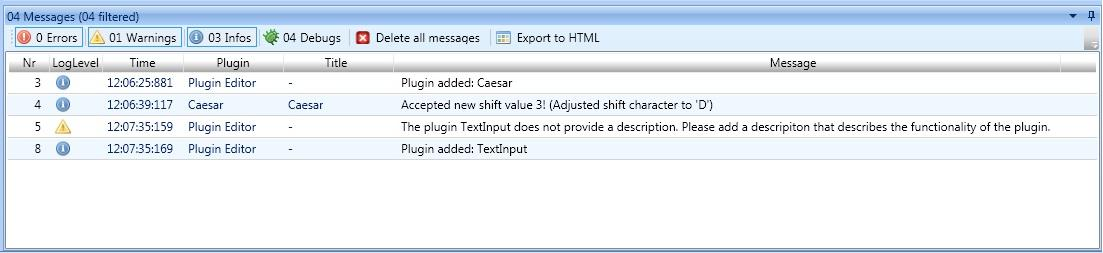
\includegraphics[width=1.00\textwidth]{figures/status_bar.jpg}
	\caption{An example status bar.}
	\label{fig:status_bar}
\end{figure}

\section{Create an editor template}
\label{DrawingTheWorkfloweOfYourPlugin}

Each plugin should have an associated workflow file to show the algorithm in action in CrypTool 2. These workflow files are saved as \textit{Compressed Workspace Manager} files with file extension \textit{.cwm}. You can view the example files from other plugins by opening any of the files in the \texttt{Templates\textbackslash} folder with CrypTool 2. Below is an example workflow (image shows old editor, but the new one looks similar). You should provide such a template .cwm file to demonstrate a typical use case of your plugin. Please place it into the \texttt{Templates\textbackslash} folder and make sure to commit the file to the SVN repository (see Section \ref{CommitingYourChanges}).

\begin{figure}[h]
	\centering
		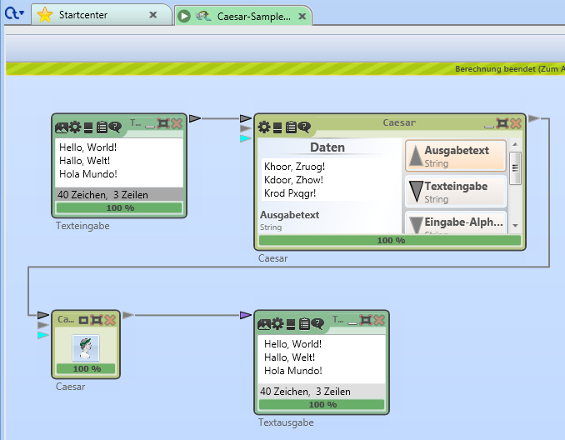
\includegraphics{figures/sample.jpg}
	\caption{A sample workflow diagram for the Caesar algorithm.}
	\label{fig:sample}
\end{figure}
